\documentclass[norsk,a4paper,12pt]{article}
\usepackage{babel}
\usepackage[utf8]{inputenc}
\usepackage[T1]{fontenc}
\usepackage{graphicx}
\graphicspath{ {../img/} }
\usepackage{array}

\begin{document}

\author{
	Jacobsen, Erlend Hernes\\
	\texttt{erljacobsen@gmail.com}
	\and
	Nielsen, Jørgen Storm\\
	\texttt{jorgenstorm.nielsen@gmail.com}
	\and
	Holmeset, Markus\\
	\texttt{markus.holmeset@gmail.com}
}
\title{Forprosjektrapport}
\date{\today}
\maketitle

\newpage

\tableofcontents

\newpage

\section{Prosjektgruppen}

\subsection{Jørgen Storm Nielsen}


\includegraphics[scale=0.5]{jorgen.png}

\textbf{Jørgen Storm Nielsen}\newline
\textbf{Tlf:} 48219443\newline
\textbf{E-post:} jørgen.s.nielsen@hiof.no\newline

Har studert Idrett ved Kristiansand Katedralskole Gimle. Studerer i dag Bachelor i Informasjonssystemer og IT-Ledelse ved Høgskolen i Østfold.

\subsection{Erlend Jacobsen}

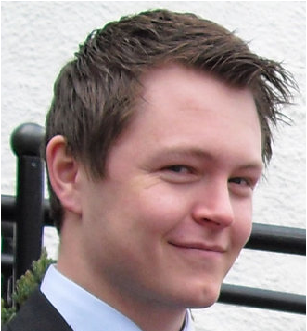
\includegraphics[scale=0.5]{erlend.png}

\textbf{Erlend Jacobsen}\newline
\textbf{Tlf:} 97777617\newline
\textbf{E-post:} erlend.h.jacobsen@hiof.no\newline

Studerte Allmenfag på Levanger VGS. Har deretter tatt befalskole og jobbet for Forsvaret. Studerer nå Bachelor i Informasjonssystemer og IT-Ledelse ved Høgskolen i Østfold.

\subsection{Markus Holmeset}


\includegraphics[scale=0.5]{markus.png}

\textbf{Markus Holmeset}\newline
\textbf{Tlf:} 99557503\newline
\textbf{E-post:} markus.holmeset@hiof.no\newline

Studerte Laboratoriefag ved Borg VGS i Sarpsborg og fagbrev tatt ved Norske Skog Saugbrugs i Halden. Studerer nå Bachelor i Dataingeniør ved Høgskolen i Østfold.


\section{Oppdragsgiver}

Oppdragsgivere i prosjektet er Dataservice og Gyldendal Undervisning. Dataservice er etablert i 1989, og er blant de største i sin bransje i Østfold. Firmaet har base i Halden, men har hele Østfold som sitt markedsområde. Selskapet leverer dataprodukter til både private og bedrifter. I tillegg til søsterselskapet Regnskapsservice, er selskapet også medeier i Odin media, et kommunikasjonsbyrå som leverer tjenester innenfor strategisk rådgivning, grafisk design og webutvikling/design.\newline

Gyldendal Undervisning er Norges største undervisningsforlag. Forlaget utgir læremidler til barnehage, grunn- og videregående skole, samt for etter- og videreutdanning innen språkopplæring og andre fagområder.

\newpage

\section{Beskrivelse av oppgaven}

\subsection{Bakgrunn}

Dataservice og Gyldendal Undervisning, heretter omtalt som oppdragsgiver,  har et ønske om å kartlegge hvilke verktøy som i dag benyttes i undervisningen av fagene IT1 og IT2. 

Bachelorgruppen synes denne oppgaven virker interessant og utfordrende oppgave, samtidig som den bidrar til å øke kvaliteten i undervisningen i fagene IT1 og IT2 i den videregående skolen. 

\subsection{Overordnet prosjektbeskrivelse}

 

Flere skoler har benyttet verktøy som Flash, PhotoShop, MySQL og Dreamweaver i IT1, mens Flash og ActionScript har blitt benyttet i IT2. 
Bruken av disse verktøyene er i endring, og oppdragsgiver ønsker en grundig kartlegging av hvilke verktøy de forsjellige skolene benytter i dag. I tillegg til kartlegging,  ønsker oppdragsgiver en anbefaling fra prosjektgruppen angående hvilken programvare og hvilke verktøy som kan benyttes i undervisningen. 

Formålet med dette prosjektet er at oppdragsgiver får en grundig analyse av hvordan  utdanningen i praksis fungerer, med tanke på bruken av de forskjellige verktøyene, samtidig som oppdragsgiver vil få en anbefaling angående hvilke verktøy som bør benyttes i undervisningen fremover.

\subsection{Rammebetingelser}

Prosjektets rammer er gitt i henhold til emnebeskrivelsen for bacheloroppgaven ved Høgskolen i Østfold, og prosjektkontrakten som er ingått mellom prosjektgruppen og oppdragsgiver. 

Prosjektets økonomi begrenser seg til prosjektgruppens tilmålte arbeidsmendge som tilsvarer ca 500 timer per student. Oppgaven skal være levert til eksamenskontoret 21 Mai 2015, som da blir prosjektets sluttdato. 

\subsection{Avgrensninger}

Selve oppgaven er avgrenset til å omhandle verktøy som benyttes, i form av programvare og programmeringsspråk. Det vil underveis i arbeidet  bli vurdert om det er andre interessante aspekter som bør bli tatt med i oppgaven. Prosjektgruppen tar høyde for dette, da det kan dukke opp informasjon underveis som er nødvendig å ta med i det videre arbeidet med oppgaven.
\section{Formål}

\subsection{Effektmål}

Prosjektet er etablert med bakgrunn i en Bachelorppgave ved Høgskolen i Østfold. Oppgaven går ut på å samle inn informasjon om hvilke verktøy som benyttes i undervisningen av fagene IT1 og IT2 ved den videregående skolen. Det overordnede målet for oppgaven, er at undervisningen i fagene IT1 og IT2 skal tilpasse seg dagens situasjon med tanke på verktøy og programmeringsspråk. Er verktøyene som blir benyttet i fagene per dags fremdeles det beste, eller er de modne for utskiftning? 

\subsection{Resultatmål}

Målet med oppgaven er å kunne legge til grunn en grundig vurdering av verktøy som blir benyttet, samt en anbefaling om eventuelle nye verktøy som kan benyttes i undervisningen av fagene. Prosjektgruppen ønsker å legge mest mulig fakta til grunn for vurderingen av dagens verktøy, i tillegg til vurdering og analyse av eventuellt nytt verkøy og programvare.

\section{Prosjektorganisering}

\subsection{Roller og ansvar}

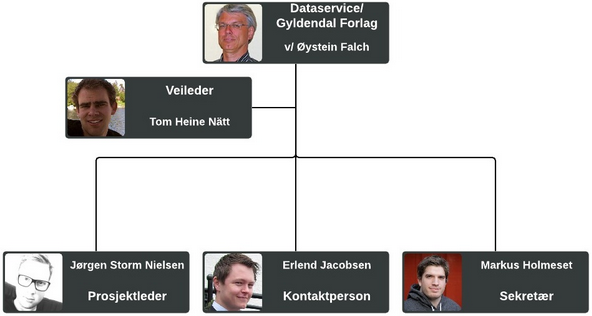
\includegraphics{prorg.png}

\noindent\textbf{Oppdragsgiver/Prosjekteier}\newline
Oppdragsgiver i prosjektet er Dataservice og Gyldendal forlag, representert ved Øystein Falch.
\newline

\noindent\textbf{Veilder}\newline
Veileder i prosjektet er Tom Heine Nätt. Rollen til veileder er å veilede prosjektgruppen, svare på spørsmål angående oppgaven og lignende. I tillegg vil veileder gi tilbakemelding underveis, samt på de tilige innleveringene.
\newline

\noindent\textbf{Prosjektleder}\newline
Prosjektleders overordnede oppgave er å sørge for at fristene i prosjektet blir fulgt, samt at utdelte oppgaver blir utført av prosjektgruppens medlemmer. 
\newline

\noindent\textbf{Kontaktperson}\newline
Kontaktpersonens oppgave er å opprettholde kontakten med oppdragsgiver og veileder, samt oppretting av  kontakt med intervjuobjekter.
\newline

\noindent\textbf{Sekretær}\newline
Sekretæren har som ansvar å føre notater på møtene, og skrive møtereferat fra møtene.


\section{Metode og Teori}

Prosjektgruppen vil benytte seg av to typer intervjuer for å finne informasjon. 
Det vil bli utført dybdeintervjuer (kvalitative) med enkelte lærere som underviser i faget, for å få en dypere forståelse for hvordan bruken av de forskjellige verktøyene fungerer i praksis, på godt og vondt.

Det vil også bli sendt ut en kvantitativ spørreundersøkelse som har som formål å gi prosjektgruppen en oversikt over læreres meninger og tanker omkring dagens verktøy. Denne spørreundersøkelsen vil bli brukt som grunnlag for mye av det videre analysearbeidet i prosjektet. Spørreundersøkelsen vil bli utarbeidet i samarbeid med oppdragsgiver og veileder.

I tillegg til intevjudelen, vil prosjektgruppen legge mye arbeid i å samle informasjon fra andre kilder. Målet med denne informasjonsinhentingen, er så kartlegge hva som er skrevet om på dette området fra før, både i nasjonalt og internasjonalt. Prosjektgruppen vil også overvære undervisningstimer i fagene for å få et lite innblikk i hvordan de forskjellige verktøyene blir benyttet i praksis. 




\newpage

\section{Prosjektplan}

\begin{center}
\begin{tabular}{ | m{5cm} | m{8cm}| m{1cm} | } 
 \hline
\textbf{Aktivitet} & \textbf{Beskrivelse} & \textbf{Dato} \\ 
\hline
Forarbeid & Sette seg inn i oppgaven og forstå problemstillingen & 9/1 \\ 
\hline
Hjemmeside & Sette opp webside for prosjektet & 9/1 \\ 
 \hline
Forprosjektrapport & Levere forprosjektrapport & 16/1 \\
\hline
Møte med lærer i faget & Organisere et møte med en lærer som har et av fagene (IT1 eller IT2) & 19/1 \\
\hline
Informasjonsinnhenting og kildesøk & Innhente relevant informasjon om emnet (artikler, bøker, undersøkelse etc) & 23/1 \\
\hline
Intervjuguide & Produsere intervjuguide for kvalitative intervjuer & 30/1 \\
\hline
Spørreundersøkelse & Spørreundersøkelse ferdigstilles & 30/1 \\
\hline
Godkjennelse av spørreundersøkelse & Spørreundersøkelse godkjennes av oppdragsgiver & 06/2 \\
\hline
Utsending av spørreundersøkelse & Spørreundersøkelsen sendes ut til lærerne & 06/2 \\
\hline
Alternativer til programvare & Finne alternativer til programvaren som benyttes i dag & 13/2 \\
\hline
Teori og metode & Teori- og metodekapittel ferdigstilles & 13/3 \\
\hline
Første versjon av hoveddokumentet & Første versjon av hoveddokumentet leveres & 13/3 \\
\hline
Konklusjon ferdig & Spørreundersøkelsen er ferdig bearbeidet og alternativer til programvare er rangert etter kriterier & 24/4 \\
\hline
Andre versjon av hoveddokument & Andre versjon av hoveddokumentet leveres & 24/4 \\
\hline
Korrekturlesing & Dokumentet er ferdig korrekturlest & 21/5 \\
\hline
Vedlegg ferdig & Vedlegg er ferdig & 21/5 \\
\hline
Innlevering av bacheloroppgave & Oppgaven leveres på eksamenskontoret & 21/5 \\
\hline
Prosjektplakat & Prosjektplakat er ferdig produsert og hengt opp & 01/6 \\
\hline
Presentasjon av bachelorprosjektet & Prosjektet presenteres for oppdragsgiver, veileder og sensor & 03/6 \\
\hline
\end{tabular}
\end{center}

\section{Leveranser}

\subsection{Gantt-diagram}

\begin{center}
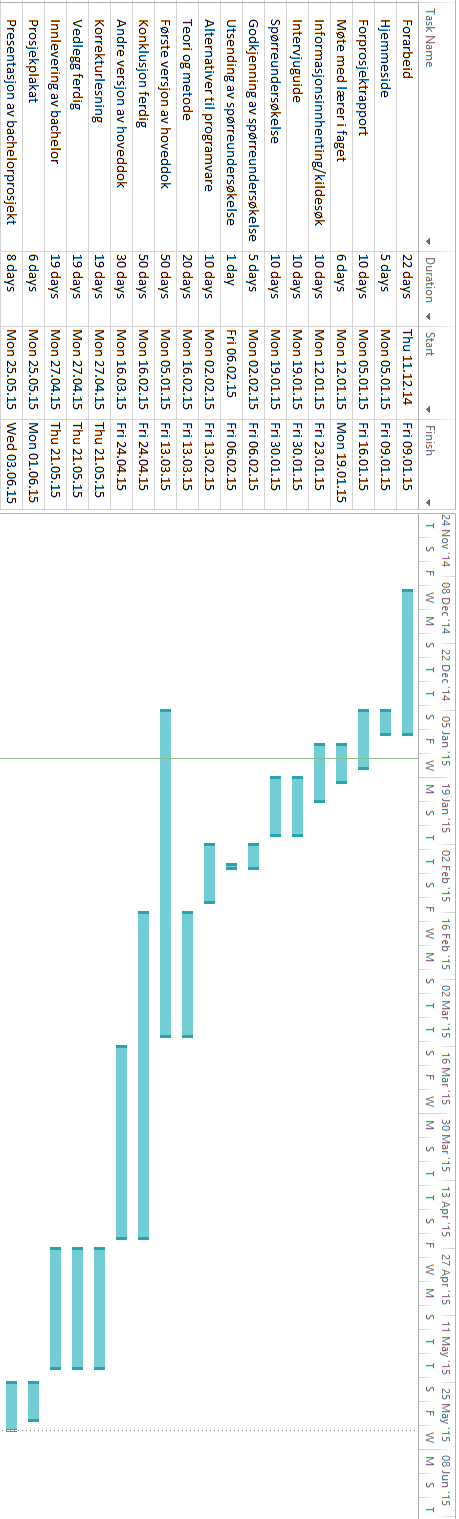
\includegraphics[scale=0.5]{gantt.png}
\end{center}

\subsection{Hovedlevereranser}

\begin{center}
\begin{tabular}{ | m{3cm} | m{8cm}| m{1cm} | } 
 \hline
\textbf{Nummer} & \textbf{Beskrivelse} & \textbf{Dato} \\ 
\hline
1 & Hjemmeside & 09/1 \\
\hline
2 & Forprosjektrapport & 16/1 \\
\hline
3 & Første versjon av hoveddokumentet & 13/3 \\
\hline
4 & Andre versjon av hoveddokumentet & 24/4 \\
\hline
5 & Levering av bacheloroppgave & 21/5 \\
\hline
6 & Prosjektplakat & 01/6 \\
\hline
7 & Presentasjon & 03/6 \\
\hline
\end{tabular}
\end{center}

\end{document}